\newif\ifdraft
\drafttrue
%\draftfalse

\ifdraft
  \documentclass[draft]{llncs}
  \usepackage{color}
  \usepackage[normalem]{ulem}
  \definecolor{green}{rgb}{.2,.8,0}
  \definecolor{blue}{rgb}{0,0,1}
  \definecolor{red}{rgb}{1,0,0}

  \usepackage[final]{graphicx}  
  
  \newcommand{\change}[1]{\textcolor{green}{#1}}
  \newcommand{\delete}[1]{\textcolor{red}{\sout{#1}}}
  \newcommand{\tbc}[1]{\textcolor{blue}{#1}}
  \newcommand{\todo}[1]{\textbf{\color{red}{TO-DO}}: #1}
  \newcommand{\mnote}[1]{\marginnote{#1}}
  
\else
  \documentclass{llncs}
  \usepackage{graphicx}
  
  \newcommand{\change}[1]{#1}
  \newcommand{\delete}[1]{}
  \newcommand{\tbc}[1]{#1}
  \newcommand{\todo}[1]{}
  \newcommand{\mnote}[1]{}
\fi

\usepackage{url}
\usepackage{alltt,verbatim}
\usepackage{soul}
\usepackage{subfig}
\usepackage{pifont}
\usepackage[utf8]{inputenc}

\usepackage[all]{xy}
\newcommand{\code}[1]{{\texttt{#1}}}

% MARGIN NOTES
\marginparwidth 1.25 true in

\newcounter{marginalnote}
\setcounter{marginalnote}{1}
\renewcommand{\themarginalnote}{\roman{marginalnote}}
\newcommand{\marginnote}[1]
           {\raisebox{1ex}{\scriptsize (\themarginalnote)}%
            \marginpar{\footnotesize\raggedright\indent
                       \raisebox{1ex}{\scriptsize (\themarginalnote)} #1}%
            \addtocounter{marginalnote}{1}}
% MARGIN NOTES

% Maude code
\usepackage[final]{listings}
\usepackage{xcolor}
\lstdefinelanguage{maude}
{
	alsoletter={\:},
    morecomment=[l]{---},
    morecomment=[l]{***},
    keywords={pr, protecting, sort, sorts, subsort, subsorts, including, class, msg, msgs, endfm, fmod, is, mod, endm, omod, endom},
    keywords=[2]{eq,  mb, ceq, if, rl, crl, else, then, fi},
    keywords=[3]{ctor, assoc, comm, gather, id\:},
    keywords=[4]{op, ops, var, vars}
}

\lstset{
  language=maude,
  basicstyle=\ttfamily\footnotesize,
  frame=tb,
	framerule=0.2pt,
  %keywordstyle=\bfseries,
	%keywordstyle=[2]\bfseries,
	%keywordstyle=[3]\bfseries,
	%keywordstyle=[4]\bfseries,
}
% Maude code

\DeclareGraphicsExtensions{.png}

\pagestyle{headings} % switches on printing of running heads
%\addtocmark{XXXX} % additional mark in the TOC

\title{The Movie Database Case: \\ A solution using the Maude-based e-Motions tool}
\titlerunning{TO-DO} % abbreviated title (for running head) also used for the TOC unless \toctitle is used

\author{Antonio~Moreno-Delgado \and Francisco~Dur\'an}
\authorrunning{Moreno et al.} %abbreviated author list (for running head)

%%%% modified list of authors for the TOC (add the affiliations)
\tocauthor{
  Antonio Moreno-Delgado (Universidad de M\'alaga),
  Francisco Dur\'an (Universidad de M\'alaga)
}

\institute{
    University of M\'alaga\\
    \email{\{amoreno,duran\}@lcc.uma.es}
    }

\begin{document}

\maketitle

\begin{abstract}

\end{abstract}

%-------------------------------------------------------------
%  INTRODUCTION
%-------------------------------------------------------------
\section{Introduction}
\label{sec:intro}
%-------------------------------------------------------------
%  INTRODUCTION
%-------------------------------------------------------------

Maude~\cite{CDELMMQ:02,CDELMMT:07-book} is an executable formal specification language based on rewriting logic, which counts with a rich set of validation and verification tools~\cite{CDELMMT:07-book,CDHLMO:07}, increasingly used as support to the development of UML, MDA, and OCL tools (see, e.g., \cite{Boronat-Meseguer:08,RRDV:07-jot,Clavel-Egea:2006}). Furthermore, Maude has demonstrated to be a good environment for rapid prototyping, and also for application development (see surveys~\cite{CDELMMT:07-book,Meseguer:2012}). 

Maude may be seen as a general framework where to develop model transformations. Thus, Meseguer and Boronat use it to implement their model transformation framework MOMENT2; Dur\'an, Vallecillo and others have used it to develop e-Motions~\cite{RiveraDV10}, a tool that supports the definition and simulation of real-time Domain-Specific Modeling Languages (DSMLs); and similar approaches have later been used to give semantics to ATL~\cite{TroyaV10} and other transformation languages. 

The e-Motions tool is a DSML and graphical framework developed for Eclipse that supports the specification, simulation, and formal analysis of real-time systems. It provides a way to graphically specify the dynamic behavior of DSMLs using their concrete syntax, making this task quite intuitive. Furthermore, e-Motions behavioral specifications are models too, so that they can be fully integrated in MDE processes.

In e-Motions, MOF metamodels are formalized in rewriting logic, providing a representation of the structural aspects of any modeling language with a MOF metamodel. Then, given a description of the behavior of such modeling language as in-place transformation rules, e-Motions may be used to define both the syntax and the operational semantics of DSMLs. Artifacts developed in e-Motions are automatically translated into Maude.

As we will see in the following sections, e-Motions provides a very rich set of features, that enables the formal and precise definition of real-time DSMLs as models in a graphical and intuitive way. It makes use of an extension of in-place model transformation with a model of timed behavior and a mechanism to state action properties. The extension is defined in such a way that it avoids artificially modifying the DSML's metamodel to include time and action properties, supports attribute computations and ordered collections, which are specified by means of OCL
expressions, thanks to mOdCL~\cite{Roldan-Duran:2008-tr}. All these features makes the language very expressive, but directly impact on performance. To gain an idea of this impact, we provide below solutions to the proposed problems both in e-Motions and directly in Maude and compare them. 

The e-Motions system documentation and several examples are available at \url{http://atenea.lcc.uma.es/e-Motions}. The Maude web site is at \url{http://maude.cs.uiuc.edu}.

\subsection{e-Motions}\label{sub:emotions}

The definition of a Domain-Specific Language (DSL) typically comprises three tasks: (i) the definition of its abstract syntax, (ii) the definition of its concrete syntax and (iii) the specification of its behavior.

In e-Motions the abstract syntax is defined by means of an Ecore metamodel, in which all the language concepts and the relations between them are specified. The concrete syntax is provided by defining the so-called Graphical Concrete Syntax (GCS). A GCS is a model (conforms the GCS metamodel) where an image is attached to each concept defined in the abstract syntax.

In e-Motions the behavior of a DSL is specified using visual graph-transformation rules. An e-Motions rule consists of a---possibly conditional---Left-Hand Side (LHS), a Right-Hand Side (RHS) and zero or more Negative Application Conditions (NACs). The LHS defines a (sub)-graph matching, optionally conditional. The RHS specifies a (sub)-graph replacement, which if the rule is applied, every object in the LHS that is not in the RHS is deleted, new objects in the RHS that are not in the LHS are created, and those objects whose attributes (or links) are changed are updated. NACs specify conditions or (sub)-graphs such that if there is a matching, the rule cannot be fired.

Figure~\ref{fig:assemble} shows an example of an e-Motions rule. The objects in both the RHS and LHS are represented by their associated images, as defined in the GCS model. Rule \code{Assemble}'s LHS defines the precondition of the rule. It models an assemble machine who needs both a head and a handle in its connected conveyor. If \code{NAC1}, stating that the current matched \code{Assemble} object is not involved in other \code{Assemble} action, is not satisfied, the rule can be applied. The rule is applied as follows. All objects in its LHS which do not appear in its RHS are deleted, i.e., objects \code{he} and \code{ha}. Those objects in its RHS which do not appear in its LHS are created, properly setting their attributes, i.e., the \code{ham} object with its three attributes. The rest of the objects remain changeless. Moreover, as e-Motions is a framework where to define real-time systems, each rule is applied in a established time, i.e. \code{[prodTime,prodTime]} in the \code{Assemble} rule. A rule with execution time \code{[0,0]} is considered instantaneous. A rule may contain zero or more local or auxiliary variables. All attribute or variable assignments and conditions are expressed using Object-Constraint Language (OCL)~\cite{ocl}.

The abstract and concrete syntax, and the behavior of a DSL are models, and the e-Motions tool has been developed following MDE principles. The Maude code corresponding to a system defined in e-Motions is generated by an ATL/TCS transformation~\cite{atl}.

\begin{figure}[htp]
  \centering
  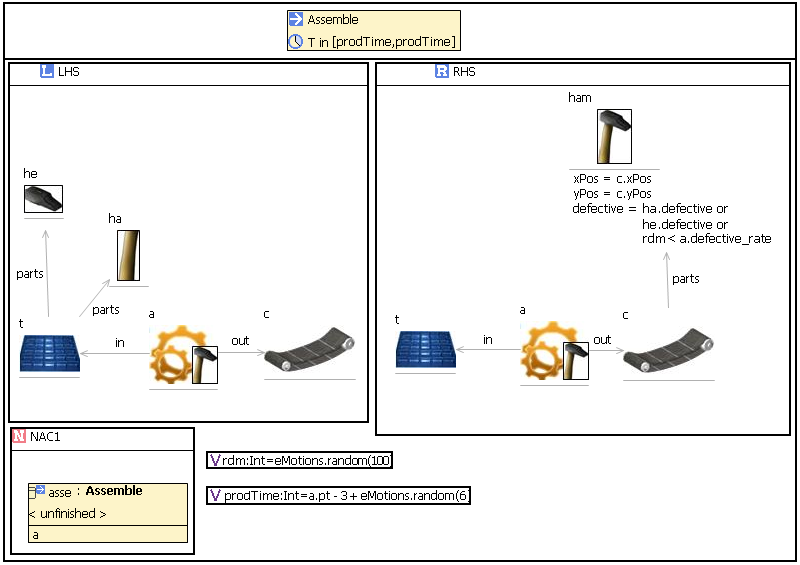
\includegraphics[width=\textwidth]{imgs/assemble}
  \caption{e-Motions \code{Assemble} rule.}\label{fig:assemble}
\end{figure}

\subsection{Rewriting Logic and Maude}

Rewriting logic (RL)~\cite{Meseguer:92-tcs} is a logic of change
that can naturally deal with state and with highly nondeterministic
concurrent computations.
In RL,  the state space of a distributed system is specified as an
algebraic data type in terms of an equational specification
$(\Sigma,E)$, where $\Sigma$ is a signature of sorts (types) and
operations, and $E$ is a set of equational axioms. The dynamics of a
system in RL is then specified by rewrite \emph{rules} of the form
$t \rightarrow t'$, where $t$ and $t'$ are $\Sigma$-terms.
This rewriting happens modulo the equations $E$, describing in fact
local transitions $[t]_E\rightarrow[t']_E$.
These rules describe the local, concurrent transitions possible in the
system, i.e. when a part of the system state fits the pattern $t$
(modulo the equations $E$)
then it can change to a new local state fitting pattern $t'$.
Notice the potential of this type of rewriting, and the very high-level of
abstraction at which systems may be specified, to perform, e.g.,
rewriting modulo associativity or associativity-commutativity.

Maude~\cite{CDELMMQ:02,CDELMMT:07-book} is a
wide spectrum programming language directly based on RL.
Thus, Maude integrates an
equational style of functional programming with RL computation.
Maude also supports the modeling of object-based systems by providing
sorts representing the essential concepts of object
(\texttt{Object}), message (\texttt{Msg}), and configuration
(\texttt{Configuration}). A configuration is a multiset of objects
and messages (with the empty-syntax, associative-commutative, union
operator \verb~__~) that represents a possible system
state.

Although the user is free to define any syntax for objects
and messages, several additional sorts and operators are introduced
as a common notation. Maude provides sorts \texttt{Oid} for object
identifiers, \texttt{Cid} for class identifiers, \texttt{Attribute}
for attributes of objects, and \texttt{AttributeSet} for multisets
of attributes (with \verb~_,_~ as union operator).
Given a class $C$ with attributes $a_i$ of types $S_i$, the objects
of this class are then record-like structures of the form

$$\texttt{<} \; O \; \texttt{:} \; C \; \texttt{|} \; a_1 \texttt{:}
v_1 \texttt{,} \; ... \texttt{,} \; a_n \texttt{:} v_n \;
\texttt{>}$$

\noindent where $O$ is the identifier of the object, and $v_i$
are the current values of its attributes (with appropriate types).
See \cite{CDELMMT:07-book} for additional details on how
object-oriented systems are represented in Maude, including
explanations on how to represent inheritance, syntax for
object-oriented modules, different forms of object communication,
etc.

The following Maude definitions specify a class
\texttt{Account} of bank accounts, with messages \verb"withdraw" and
\verb"transfer" to operate with such bank accounts. The
\verb"Account" class is defined with a single attribute
\verb"balance", of sort \verb"Int", representing the balance of an
account. The \verb"withdraw" message has two parameters, namely the
addressee of the message and the amount of money to withdraw from
the account. The \verb"transfer" message will make the amount of
money specified as its third argument to be transferred from the
account given as first argument to the one given as second argument.

{\small
\begin{verbatim}
  sort Account .
  subsort Account < Cid .
  op Account : -> Account .
  op balance :_ : Int -> Attribute .
  op withdraw : Oid Int -> Msg .
  op transfer : Oid Oid Int -> Msg .
\end{verbatim}
}

\noindent Rules \verb"debit" and  \verb"transfer" below represent local
transitions of the system that specify the behavior of bank accounts
upon the reception of such messages. E.g., if an \verb"Account"
object receives a \verb"withdraw" message and the amount of money to
withdraw is smaller or equal than the balance of the account
receiving the message, then the message is `consumed' and the
balance of the account is decremented is such an amount. Notice the
synchronization of \verb"Account" objects in the \verb"transfer"
rule.

{\small
\begin{verbatim}
  vars A B : Oid .
  vars BalA BalB M : Int .

  crl [debit] :
    < A : Account | balance : BalA >
    withdraw(A, M)
    => < A : Account | balance : BalA - M >
    if BalA >= M .
  crl [tranfer] :
    < A : Account | balance : BalA >
    < B : Account | balance : BalB >
    withdraw(A, M)
    => < A : Account | balance : BalA - M >
       < B : Account | balance : BalB + M >
    if BalA >= M .
\end{verbatim}
}

\noindent Notice that, since the \verb"__" operator is declared associative,
commutative, and with identity element, we do not need to worry about the order
in which objects and messages appear in the rules.
And since rules describe local transitions, we do not need to worry
about the rest of the objects and messages in the configuration either.

Well-formedness of objects may be automatically checked by Maude's typing system.
For example, we can add declarations constraining \verb"Account" objects:

{\small
\begin{verbatim}
  sort AccountObject .
  subsort AccountObject < Object .

  var O : Oid .
  var Bal : Int .

  mb < O : Account | balance : Bal > : AccountObject .
\end{verbatim}
}

\noindent Notice that with these declarations, an object
  \verb"< O : Account | >"
is a valid term of sort \verb"Object", but since the membership cannot be applied on it,
it is not of type \verb"AccountObject".



%-------------------------------------------------------------
% SOLUTIONS
%-------------------------------------------------------------
\section{Solution}
\label{sec:solution}

%-------------------------------------------------------------
% SOLUTIONS
%-------------------------------------------------------------

We are presenting two solutions for the different tasks, one graphical solution using e-Motions, and another one using directly Maude. Each task is solved by defining respective DSLs, which share their abstract and concrete syntaxes. The abstract syntax used is the one provided at~\cite{imdbsources} --- we will see below that some of the tasks have required extensions of this common syntax. The main differences between the DSLs defined for the different tasks is in their  concrete behaviors describing what need to be done in each case, that is, the rewrite rules defining the behavior depends on the concrete task and its solution. 

The e-Motions description of the different tasks is then transformed into a Maude specification and executed in Maude. We show how the formal tools available in Maude allow us to check the transformations carried out. Specifically, we will illustrate the use of Maude's reachability analysis capabilities to check that no undesired situation is reached along the execution. 

Although the expressiveness of e-Motions is very welcome in complex problems, thanks to its capabilities to express problems visually, very intuitively and in a language very close to the problem domain, the overhead to be paid in cases like the ones at hand is too high. Specifically, the generality provided by its support for OCL expressions and time requirements, makes that the Maude code generated by the e-Motions tool is not as time performant as we would like. However, the general purpose rewrite-modulo engine at the core of Maude may also be used as a transformation language. Thus, together with the e-Motions solution we present a optimized Maude solution for each task.  

As we will see below, the Maude version of the transformation closely follows the transformations provided in e-Motions, were all rewrite rules are \textit{instantaneous} and expressions are solved directly by Maude built-in types instead of by the OCL interpreter \cite{mOdCL}. Indeed, for problems as simple as the ones at hand, we will see that the representation distance between Maude and e-Motions to the problem domain would be almost as small, making both solutions very appropriate. Although a more in deep analysis of the problem at hand would most probably have allowed us to even improve the numbers obtained, we have preferred to keep the specification clear and intuitive.



%%%%%%%%%%%%%%%%%%%%%%%%%%%%%%%%%%%%%%%%%%%%%%%%%%%%%%%%%%%%%%%
%\subsection{Task 1}
%\label{sub:task1}
%%%%%%%%%%%%%%%%%%%%%%%%%%%%%%%%%%%%%%%%%%%%%%%%%%%%%%%%%%%%%%%

Task 1 comprises the generation of synthetic models (conforming the movie database metamodel~\cite{imdbcase}) from an input parameter $N \geq 0$. We first present an e-Motions solution and then a Maude solution. 


%%%%%%%%%%%%%%%%%%%%%%%%%%%%%%%%%%%%%%%%%%%%%%%%%%%%%%%%%%%%%%%
\subsubsection{e-Motions-based solution.}

Following an e-Motions based approach, we define the abstract and concrete syntax and the behavior of our so-called \textit{Task 1 DSL}. Taking a parameter $N$ as input model, \textit{Task 1 DSL} generates a model containing synthetic data.

As it has been introduced in Section~\ref{sub:emotions}, the abstract syntax of a DSL is given in e-Motions by means of an Ecore metamodel. Since we model the solution of the task as a model that evolves until reaching its final solution, we take as metamodel the one provided beforehand in~\cite{imdbsources}, which we call \textit{Movies MM}, extended with a \code{Parameter} concept. This results in a so-called \textit{Movies* MM}. The class \code{Parameter} has two integer attributes, namely \code{nP} and \code{nN}, which represent positive graphs and negative graphs, respectively, for the generation following Henshing graphs~\cite{Henshin:10}.

For the concrete syntax, Figure~\ref{fig:concreteSyntax} shows how an image has been attached to each concept modeled in the Movies* MM. 

The behavior of this \textit{Task 1 DSL} is then given by means of two in-place transformation rules: \code{createPositive} and \code{createNegative}. Figure~\ref{fig:createPositive} shows the \code{createPositive} rule, which takes an object \code{p} of type \textit{Parameter}, with \textit{nP} attribute greater or equal than $0$, and produces synthetic data conforming to the Henshing rules~\cite{Henshin:10}. Figure~\ref{fig:createNegative} shows the \code{createNegative} rule, which is analogously defined.

\begin{figure}[tb]
  \subfloat[Actor.\label{fig:actor}]{
    \makebox[60px][c]{
\includegraphics[scale=1]{imgs/actor}}
  }
  \hfill
  \subfloat[Actress.\label{fig:actress}]{
    \makebox[60px][c]{
\includegraphics[scale=1]{imgs/actress}}
  }
  \hfill
  \subfloat[Movie.\label{fig:movie}]{
    \makebox[60px][c]{
\includegraphics[scale=1]{imgs/movie}}
  }
  \hfill
  \subfloat[Couple.\label{fig:couple}]{
    \makebox[60px][c]{
\includegraphics[scale=1]{imgs/couple}}
  }
  \hfill
  \subfloat[Parameter.\label{fig:parameter}]{
    \makebox[60px][c]{
\includegraphics[scale=1]{imgs/parameter}}
  }
  \caption{Concrete syntax for \textit{Movies* MM}.}
  \label{fig:concreteSyntax}
\end{figure}

\begin{figure}[tb]
  \subfloat[The \code{createPositive} rule.\label{fig:createPositive}]{%
    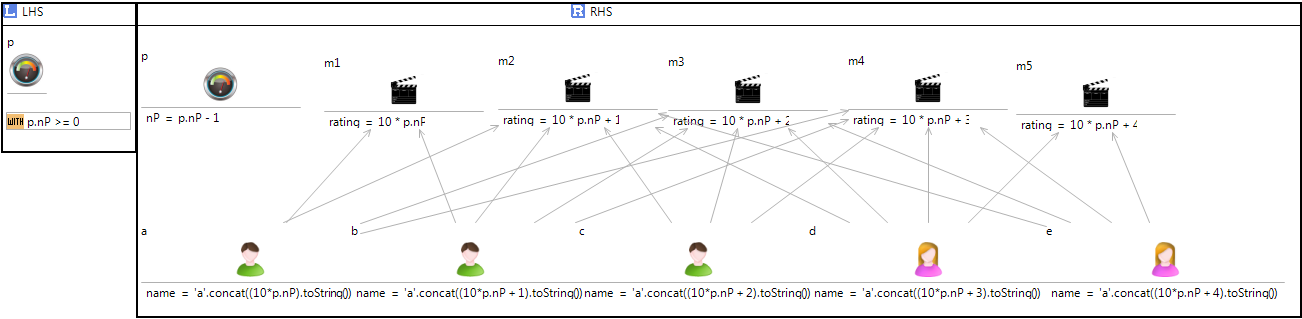
\includegraphics[width=\textheight, angle=90]{imgs/createPositiveRule}
  }
  \hfill
%  \subfloat[Rules' headers.]{
%    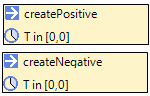
\includegraphics[width=0.2\textwidth]{imgs/headersCreate}
%  }
%  \hfill
  \subfloat[The \code{negativePositive} rule.\label{fig:createNegative}]{%
    \ \ \ \ 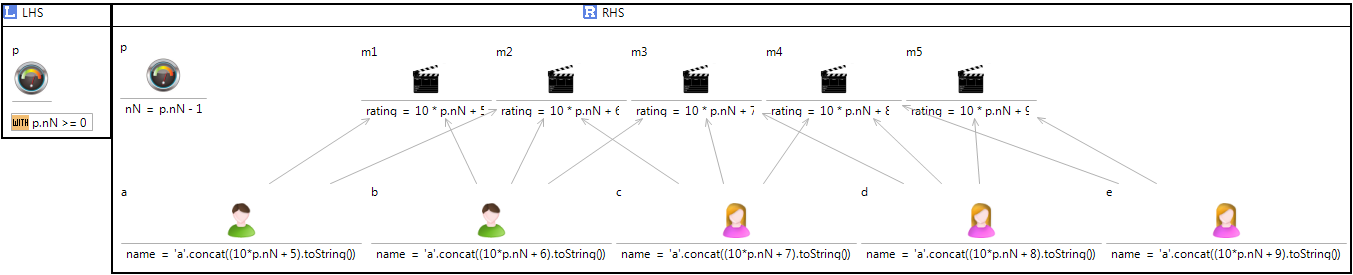
\includegraphics[width=\textheight, angle=90]{imgs/createNegativeRule}\ \ \ \ 
  }
  \caption{Task 1 rules. \label{fig:task1}}
\end{figure}

Once the syntax and the behavior of the system has been coded, the user may specify a model, which conforms to \textit{Movies* MM}, containing an object \code{Parameter} with its two attributes \code{nP} and \code{nN} properly set. This model is used as initial model of the execution.

Please, note that this solution is really close to the problem specification in~\cite{imdbcase}. Figure~\ref{fig:task1} and~\cite[Figure~2]{imdbcase}, specifying the data generation, are almost the same. This demonstrates how close the solution by e-Motions is to the problem domain, and how convenient its graphical facilities are.

\subsubsection{Maude version.}
Our Maude-based solution for Task 1 consists of an object-based Maude specification, consisting of two modules: the \code{MOVIES@MM} module defining the classes structure, and the \code{TASK1} module defining the rewrite rules to calculate the solution. As in the e-Motions solution, we have two rewrite rules: \code{createPositive} and \code{createNegative}. Listing \ref{lst:createPositive} shows the \code{createPositive} Maude rule, that takes the \code{createPositive(s(N:Nat))} message and a \code{freshOid} auxiliary message---used to create new object identifiers---and returns such a object configuration conforming the Henshin specification~\cite{imdbcase}. A similar rule generates the negative cases. Please notice that the Maude version is very much like the e-Motions version. In fact, the former is almost the textual version of the latter. 

\begin{lstlisting}[caption=\code{createPositive} Maude rule., label=lst:createPositive]
rl [createPositive] :
  createPositive(s(N))
  freshOid(N')
=>
  createPositive(N)
  < N'     : Movie | rating: (10.0 * float(N)) >
  < N' + 1 : Movie | rating: (10.0 * float(N) + 1.0) >
  < N' + 2 : Movie | rating: (10.0 * float(N) + 2.0) >
  < N' + 3 : Movie | rating: (10.0 * float(N) + 3.0) >
  < N' + 4 : Movie | rating: (10.0 * float(N) + 4.0) >
  
  < N' + 5 : Actor | name: ("a" + string(10 * N, 10)),
                   movies: (N', N' + 1, N' + 2, N' + 3) >
  < N' + 6 : Actor | name: ("a" + string(10 * N + 1, 10)),
                   movies: (N', N' + 1, N' + 2) >
  < N' + 7 : Actor | name: ("a" + string(10 * N + 2, 10)),
                   movies: (N' + 1, N' + 2, N' + 3) >
  < N' + 8 : Actress | name: ("a" + string(10 * N + 3, 10)),
                   movies: (N' + 1, N' + 2, N' + 3, N' + 4) >
  < N' + 9 : Actress | name: ("a" + string(10 * N + 4, 10)),
                   movies: (N' + 1, N' + 2, N' + 3, N' + 4) >
  freshOid(N' + 10) .
\end{lstlisting}

\subsubsection{Execution performance for both solutions.}

Table \ref{table:task1} shows the number of rewrites and execution times for both solutions. As explained above, the the execution times for the Maude specification obtained from the e-Motions definition grows very quickly. Notice that, although the number of rewrites grows linearly with respect to $N$, the time is exponential due to the infrastructure to deal with all the extra features in e-Motions. However, notice how the number of rewrites for the Maude solution grows linearly as well, but in this case the execution times grows more slowly, being able to handle problems of much bigger sizes.

\begin{table*}[tb]
\renewcommand{\tabcolsep}{6pt}
\renewcommand{\arraystretch}{1.2}
	\caption{Times for the e-Motions and Maude solutions to Task 1}
	\label{table:task1}
    \centering
	\begin{tabular}[tb]{r|r|r|r|r|}
	\hline
	    & \multicolumn{2}{|c|}{e-Motions} & \multicolumn{2}{|c|}{Maude} \\
	\hline
	$N$ & Time (s) & \# Rewrites & Time (s) & \# Rewrites \\
	\hline
	1    &       &           & 0.0 &       68 \\
	2    &   0.0 &     4,910 && \\
	10   &   0.0 &    24,334 && \\
	20   &   0.0 &    48,614 && \\
	100  &   0.6 &   242,854 && \\
	1000 &  55.7 & 2,428,054 &   1.9 &  67,001 \\
	2000 & 395.0 & 4,856,054 &  12.7 & 134,001 \\
	3000 &       &           &  33.9 & 201,001 \\
	4000 &       &           &  64.1 & 268,001 \\
	5000 &       &           & 104.4 & 335,001 \\
	6000 &       &           & 109.6 & 402,001 \\
	7000 &       &           & 144.5 & 469,001 \\
	\hline 
	\end{tabular}
	\vspace{1cm}
\end{table*}

\subsubsection{On the correctness of the transformation}

Maude provides a whole formal environment where we can perform proofs of correctness of our solution. In addition to tools to verify the termination, confluence, etc. of our rewrite systems, Maude provides a reachability analysis tool and a model checker, which are particularly attractive for performing checks on the correctness of systems. Let us consider here the Maude \code{search} command, which allows us to explore the whole reachable state space, or up to a given depth, looking for states satisfying a given condition. 

For instance, following the results given in~\cite{imdbcase}, for some $N$, the above rules \code{createPositive} and \code{createNegative} create $20N$ objects, specifically, $10N$ movies, $5N$ actresses, and $5N$ actors. We could check that the solution found satisfies this condition, but we can do something more interesting by checking that no final reachable state fails to satisfy it. Of course, if the rewrite system is confluent and terminating the solution would be unique. 

Given the \code{numOfMovies} operation, which takes an object configuration as input and returns the number of movies in it, we may look for those final states in which the number of movies will be different than $10N$ (being N the parameter of the operation \code{createExample}):
\begin{verbatim}
  search createPositive(8) createNegative(8) freshOid(0) 
    =>! C:Configuration
    such that numOfMovies(C:Configuration) =/= 10 * 8 .
\end{verbatim}

The arrow \code{=>!} means that it search for final states, that is, states that cannot be further rewritten, starting from the given initial configuration, that satisfy the given condition. Maude returns no solution for the above code, that means all final states reached have exactly 10 movies:
\begin{verbatim}
  No solution.
\end{verbatim}
%  states: 5  rewrites: 180 in 0ms cpu (0ms real)


%\begin{table*}
%\renewcommand{\tabcolsep}{6pt}
%\renewcommand{\arraystretch}{1.2}
%	\caption{e-Motions times for Task 1.}
%	\label{table:emotionstask1}
%\centering
%	\begin{tabular}[tb]{r|r|r|}
%	$N$ & Time (s) & \# Rewrites \\
%	\hline
%	2 & 0.0 & 4,910 \\
%	10 & 0.0 & 24,334 \\
%	20 & 0.0 & 48,614 \\
%	100 & 0.6 & 242,854 \\
%	1000 & 55.7 & 2,428,054 \\
%	2000 & 395.0 & 4,856,054 \\
%	\hline 
%	\end{tabular}
%	\vspace{1cm}
%\end{table*}
%
%\begin{table}
%  \begin{center}
%	\begin{tabular}{r r r}
%	$N$ & Time (s) & \# Rewrites \\
%	\hline
%	1 & 0.0 & 68 \\
%	1000 & 1.9 & 67,001 \\
%	2000 & 12.7 & 134,001 \\
%	3000 & 33.9 & 201,001 \\
%	4000 & 64.1 & 268,001 \\
%	5000 & 104.4 & 335,001 \\
%	6000 & 109.6 & 402,001 \\
%	7000 & 144.5 & 469,001 \\
%	\hline \\
%	\end{tabular}
%	\caption{Maude times for Task 1.}\label{table:maudetask1}
%	\end{center}
%\end{table}
%
%
%


%%%%%%%%%%%%%%%%%%%%%%%%%%%%%%%%%%%%%%%%%%%%%%%%%%%%%%%%%%%%%%%
%\subsection{Task 2}
%\label{sub:task2}

Task 2 consists in finding all `couples' from a given model, given that two persons are a `couple' if they played together in at least three movies~\cite{imdbcase}. Couples are to be obtained using either from the model obtained in Task 1 or from the IMBd database~\cite{imdbsources}. Once again, we present solutions using e-Motions and Maude.

\subsubsection{e-Motions-based solution}

The solution for this task is implemented with one single rule, \code{createCouple}, shown in Fig.~\ref{fig:createCouple}. \code{Person} objects are shown using square shapes because \code{Person} is an abstract class and it does not have attached image. The \code{createCouple} rule models the creation of a couple by taking two persons and generating a couple with them. The rule has two conditions: a positive condition stating that \textit{``the number of movies in the intersection between the movies of \code{per1} and \code{per2} is greater or equal than 3''}; and a negative condition, the \code{coupleHasNotBeenCreated} NAC, requiring that the couple does not exists yet. 

Although very intuitive and simple, this solution is computationally very expensive. Notice that the number of matchings in the LHS of the rule is combinatorial, leaving all the task to the evaluation of the conditions to accept or discard the couples. 

\begin{figure}[htp]
  \centering
  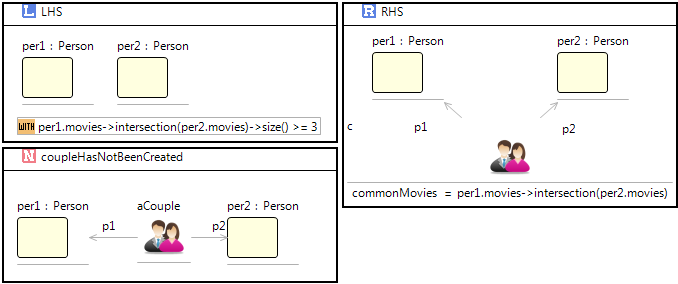
\includegraphics[width=\textwidth]{imgs/ruleCouples}
  \caption{\code{createCouple} rule.}\label{fig:createCouple}
\end{figure}

\begin{table*}[tb]
\renewcommand{\tabcolsep}{6pt}
\renewcommand{\arraystretch}{1.2}
    \centering
	\begin{tabular}[tb]{r|r|r|}
	$N$ & Time (s) & \# Rewrites \\
	\hline
	2 & 0.7 & 524,781 \\
	10 & 46.7 & 19,453,091 \\
	20 & 660.1 & 161,741,321 \\
	\hline \\
	\end{tabular}
	\caption{e-Motions times for Task 2 First Version.}\label{table:emotionstask1}
\end{table*}

We have implemented another solution in which we limit the number of matchings using a very simple algorithm: For each person, we iterate on the rest of persons looking for couples.  
%\begin{enumerate}
%  \item We split \code{Person}s and \code{Movie}s into separate configurations.
%  \item We fix a \code{Person}.
%  \item Given a \code{Person}, we look for all couples.
%  \item Whether the current \code{Person} set has been gone over all the other persons, we set the next person, and the current person is move to the resulting collection.
%\end{enumerate}
With this algorithm, the number of persons to match as candidate couple decreases significantly. To model this solution, we extend the metamodel and its concrete syntax with a so-called \code{Collection} concept. This class has three attributes, namely \code{people}, with the set of persons to be handled, \code{fixedPerson}, to iterate on each person, and \code{peopleDealtWith}, to keep the persons already considered to create a couple with the current `fixed person'. Figures~\ref{fig:initialRule}-\ref{fig:nextPerson} show the rules specifying this solution: 
\begin{itemize}
\item
Rule \code{initialRule} in Figure~\ref{fig:initialRule} initializes the collection object assigning the set of all actors and actresses to its \code{people} attribute (the other attributes get default values). This rule is only fired if there is no collection object in the model. 
\item
Rule \code{fixPerson} in Figure~\ref{fig:fixPerson} takes a person from the \code{people} set and takes it as \code{fixedPerson}. Notice that \code{p} is removed from the \code{people} set.
\item
Rules \code{doingCouples-AreCouple} and \code{doingCouples-AreNotCouple} in Figures~\ref{fig:areCouple} and \ref{fig:areNotCouple} take a person from the set \code{people} and the \code{fixedPerson} and make a couple if the number of movies they share is greater or equal than three. In both cases the person considered is passed to the \code{peopleDealtWith} set. 
\end{itemize}
When all persons has been considered as couple of the current \code{fixedPerson}, the \code{nextPerson} rule, takes the \code{peopleDealtWith} as new \code{people} set. 

\begin{figure}[htp]
  \centering
  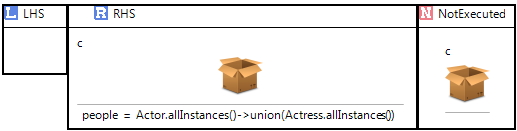
\includegraphics[width=.8\textwidth]{imgs/initialRule}
  \caption{\code{initialRule} rule.}\label{fig:initialRule}
\end{figure}

\begin{figure}[htp]
  \centering
  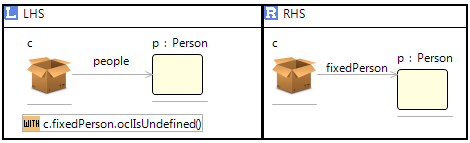
\includegraphics[width=.75\textwidth]{imgs/fixPerson}
  \caption{\code{fixPerson} rule.}\label{fig:fixPerson}
\end{figure}

\begin{figure}[htp]
  \centering
  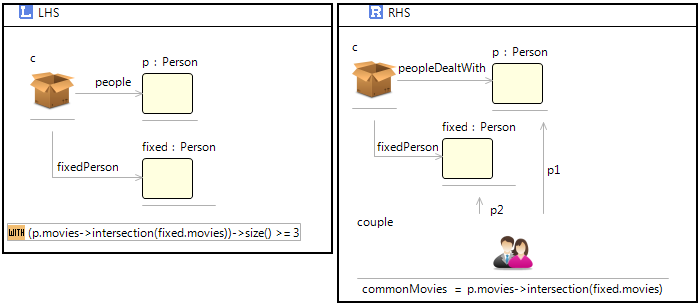
\includegraphics[width=\textwidth]{imgs/areCouple}
  \caption{\code{doingCouples-AreCouple} rule.}\label{fig:areCouple}
\end{figure}

\begin{figure}[htp]
  \centering
  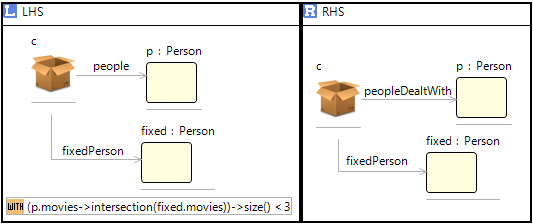
\includegraphics[width=.8\textwidth]{imgs/areNotCouple}
  \caption{\code{doingCouples-AreNotCouple} rule.}\label{fig:areNotCouple}
\end{figure}

\begin{figure}[htp]
  \centering
  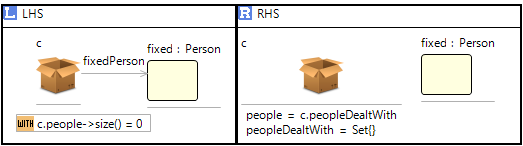
\includegraphics[width=.9\textwidth]{imgs/nextPerson}
  \caption{\code{nextPerson} rule.}\label{fig:nextPerson}
\end{figure}

%!TEX encoding = UTF-8 Unicode\begin{table}
%  \begin{center}
%	\begin{tabular}{r r r}
%	$N$ & Time (s) & \# Rewrites \\
%	\hline
%	2 & 30.105 & 27725365 \\
%	\hline \\
%	\end{tabular}
%	\caption{e-Motions times for Task 2 Second Version.}\label{table:emotionstask22}
%	\end{center}
%\end{table}


\subsubsection{Maude-based solution.}

Again, we specify directly in Maude both solutions. As for Task 1, the solutions match very closely their e-Motions counterparts. 

The Maude solution for the first alternative solution to Task 1 is shown in Listing~\ref{lst:oneRuleCouples}. The rules takes two persons and creates a new couple if they share three movies and such couple has not been previously created. Some numbers for its execution are shown in Table~\ref{table:maudetask21}.
 
\begin{lstlisting}[caption=\code{createCouples} Maude rule., label=lst:oneRuleCouples]
crl [findCouples] :
 { freshOid(N) findCouples
   < O1 : V1:Person | movies : MS1, Atts1 >
   < O2 : V2:Person | movies : MS2, Atts2 > 
   Conf }
=>
 { freshOid(s(N)) findCouples
   < O1 : V1:Person | movies : MS1, Atts1 >
   < O2 : V2:Person | movies : MS2, Atts2 >
   < N : Couple | 
           commonMovies : (intersection((MS1), (MS2))),
           p1 : O1, p2 : O2 > 
   Conf }
if | intersection((MS1), (MS2)) | >= 3
/\ not coupleInConf(C, Conf) .
\end{lstlisting}

\begin{table*}[htb]
\renewcommand{\tabcolsep}{6pt}
\renewcommand{\arraystretch}{1.2}
    \centering
	\begin{tabular}{r r r}
	$N$ & Time (s) & \# Rewrites \\
	\hline
	1 & 0.0 & 8,680 \\
	5 & 0.5 & 1,343,000 \\
	10 & 5.0 & 11,020,000 \\
	20 & 66.3 & 89,276,000 \\
	30 & 314.0 & 302,568,000 \\
	\hline \\
	\end{tabular}
	\caption{Maude times for Task 2 First Version.}\label{table:maudetask21}
\end{table*}

As for e-Motions, the second solutions consists of several rules. In this case, our collection object is model by an operator \code{\{\_\}\{\_\}\{\_\}\{\_\}\{\_\}\{\_\}} representing an object with six attributes as its e-Motions counterpart: the first argument takes the starting argument, the second the people set, the movies set, the dealt people, the fixed person on which to iterate, and the result configuration. We show in Listing~\ref{lst:task2SecondVersion} the code for the \code{doingPairs} rule. In the case of Maude, we only need one rule to consider the positive and negative cases. The number of rewrites and execution times for executions of different sizes are shown in Table~\ref{table:maudetask22}.

\begin{lstlisting}[caption=\code{doingCouples} Maude rule., label=lst:task2SecondVersion]

rl [doingPairs] :
  < { none }
    { < O1 : V1@Person | movies : MS1, Atts1 >  C1 }
    { C2 }
    { C3 }
    { < O2 : V2@Person | movies : MS2, Atts2 > }
    { freshOid(New) C4 } >
=> 
  < { none }
    { C1 }
    { C2 }
    { < O1 : V1@Person | movies : MS1, Atts1 > C3 }
    { < O2 : V2@Person | movies : MS2, Atts2 > }
    { if | intersection(MS1, MS2) | >= 3 
      then < New : Couple | p1 : O1, p2 : O2, 
              commonMovies : intersection(MS1, MS2), 
              avgRating : 0.0 >
           freshOid(s New)
      else freshOid(New)
      fi 
      C4 } > .
\end{lstlisting}

\begin{table*}[htb]
\renewcommand{\tabcolsep}{6pt}
\renewcommand{\arraystretch}{1.2}
    \centering
	\begin{tabular}{r r r}
	$N$ & Time (s) & \# Rewrites \\
	\hline
	1 & 0.0 & 831 \\
	10 & 0.1 & 82,983 \\
	100 & 8.9 & 8,299,803 \\
	200 & 68.3 & 33,199,603 \\
	300 & 242.9 & 74,699,403 \\
	400 & 640.1 & 132,799,203 \\
	\hline \\
	\end{tabular}
	\caption{Maude times for Task 2 Second Version.}\label{table:maudetask22}
\end{table*}


%-------------------------------------------------------------
% CONCLUSIONS
%-------------------------------------------------------------
\section{Conclusions}

%-------------------------------------------------------------
% CONCLUSIONS
%-------------------------------------------------------------
%\section{Conclusions}


\bibliographystyle{splncs03}
\bibliography{TTC14}
\providecommand{\url}[1]{\texttt{#1}}
\end{document}
